\documentclass[]{elsarticle} %review=doublespace preprint=single 5p=2 column
%%% Begin My package additions %%%%%%%%%%%%%%%%%%%
\usepackage[hyphens]{url}

  \journal{An awesome journal} % Sets Journal name


\usepackage{lineno} % add
\providecommand{\tightlist}{%
  \setlength{\itemsep}{0pt}\setlength{\parskip}{0pt}}

\usepackage{graphicx}
\usepackage{booktabs} % book-quality tables
%%%%%%%%%%%%%%%% end my additions to header

\usepackage[T1]{fontenc}
\usepackage{lmodern}
\usepackage{amssymb,amsmath}
\usepackage{ifxetex,ifluatex}
\usepackage{fixltx2e} % provides \textsubscript
% use upquote if available, for straight quotes in verbatim environments
\IfFileExists{upquote.sty}{\usepackage{upquote}}{}
\ifnum 0\ifxetex 1\fi\ifluatex 1\fi=0 % if pdftex
  \usepackage[utf8]{inputenc}
\else % if luatex or xelatex
  \usepackage{fontspec}
  \ifxetex
    \usepackage{xltxtra,xunicode}
  \fi
  \defaultfontfeatures{Mapping=tex-text,Scale=MatchLowercase}
  \newcommand{\euro}{€}
\fi
% use microtype if available
\IfFileExists{microtype.sty}{\usepackage{microtype}}{}
\bibliographystyle{elsarticle-harv}
\usepackage{color}
\usepackage{fancyvrb}
\newcommand{\VerbBar}{|}
\newcommand{\VERB}{\Verb[commandchars=\\\{\}]}
\DefineVerbatimEnvironment{Highlighting}{Verbatim}{commandchars=\\\{\}}
% Add ',fontsize=\small' for more characters per line
\usepackage{framed}
\definecolor{shadecolor}{RGB}{248,248,248}
\newenvironment{Shaded}{\begin{snugshade}}{\end{snugshade}}
\newcommand{\AlertTok}[1]{\textcolor[rgb]{0.94,0.16,0.16}{#1}}
\newcommand{\AnnotationTok}[1]{\textcolor[rgb]{0.56,0.35,0.01}{\textbf{\textit{#1}}}}
\newcommand{\AttributeTok}[1]{\textcolor[rgb]{0.77,0.63,0.00}{#1}}
\newcommand{\BaseNTok}[1]{\textcolor[rgb]{0.00,0.00,0.81}{#1}}
\newcommand{\BuiltInTok}[1]{#1}
\newcommand{\CharTok}[1]{\textcolor[rgb]{0.31,0.60,0.02}{#1}}
\newcommand{\CommentTok}[1]{\textcolor[rgb]{0.56,0.35,0.01}{\textit{#1}}}
\newcommand{\CommentVarTok}[1]{\textcolor[rgb]{0.56,0.35,0.01}{\textbf{\textit{#1}}}}
\newcommand{\ConstantTok}[1]{\textcolor[rgb]{0.00,0.00,0.00}{#1}}
\newcommand{\ControlFlowTok}[1]{\textcolor[rgb]{0.13,0.29,0.53}{\textbf{#1}}}
\newcommand{\DataTypeTok}[1]{\textcolor[rgb]{0.13,0.29,0.53}{#1}}
\newcommand{\DecValTok}[1]{\textcolor[rgb]{0.00,0.00,0.81}{#1}}
\newcommand{\DocumentationTok}[1]{\textcolor[rgb]{0.56,0.35,0.01}{\textbf{\textit{#1}}}}
\newcommand{\ErrorTok}[1]{\textcolor[rgb]{0.64,0.00,0.00}{\textbf{#1}}}
\newcommand{\ExtensionTok}[1]{#1}
\newcommand{\FloatTok}[1]{\textcolor[rgb]{0.00,0.00,0.81}{#1}}
\newcommand{\FunctionTok}[1]{\textcolor[rgb]{0.00,0.00,0.00}{#1}}
\newcommand{\ImportTok}[1]{#1}
\newcommand{\InformationTok}[1]{\textcolor[rgb]{0.56,0.35,0.01}{\textbf{\textit{#1}}}}
\newcommand{\KeywordTok}[1]{\textcolor[rgb]{0.13,0.29,0.53}{\textbf{#1}}}
\newcommand{\NormalTok}[1]{#1}
\newcommand{\OperatorTok}[1]{\textcolor[rgb]{0.81,0.36,0.00}{\textbf{#1}}}
\newcommand{\OtherTok}[1]{\textcolor[rgb]{0.56,0.35,0.01}{#1}}
\newcommand{\PreprocessorTok}[1]{\textcolor[rgb]{0.56,0.35,0.01}{\textit{#1}}}
\newcommand{\RegionMarkerTok}[1]{#1}
\newcommand{\SpecialCharTok}[1]{\textcolor[rgb]{0.00,0.00,0.00}{#1}}
\newcommand{\SpecialStringTok}[1]{\textcolor[rgb]{0.31,0.60,0.02}{#1}}
\newcommand{\StringTok}[1]{\textcolor[rgb]{0.31,0.60,0.02}{#1}}
\newcommand{\VariableTok}[1]{\textcolor[rgb]{0.00,0.00,0.00}{#1}}
\newcommand{\VerbatimStringTok}[1]{\textcolor[rgb]{0.31,0.60,0.02}{#1}}
\newcommand{\WarningTok}[1]{\textcolor[rgb]{0.56,0.35,0.01}{\textbf{\textit{#1}}}}
\usepackage{longtable}
\usepackage{graphicx}
\ifxetex
  \usepackage[setpagesize=false, % page size defined by xetex
              unicode=false, % unicode breaks when used with xetex
              xetex]{hyperref}
\else
  \usepackage[unicode=true]{hyperref}
\fi
\hypersetup{breaklinks=true,
            bookmarks=true,
            pdfauthor={},
            pdftitle={An R Markdown template for report},
            colorlinks=true,
            urlcolor=blue,
            linkcolor=magenta,
            pdfborder={0 0 0}}
\urlstyle{same}  % don't use monospace font for urls

\setcounter{secnumdepth}{5}
% Pandoc toggle for numbering sections (defaults to be off)

\newlength{\cslhangindent}
\setlength{\cslhangindent}{1.5em}
\newenvironment{cslreferences}%
  {\setlength{\parindent}{0pt}%
  \everypar{\setlength{\hangindent}{\cslhangindent}}\ignorespaces}%
  {\par}

% Pandoc header



\usepackage{amsthm}
\newtheorem{theorem}{Theorem}[section]
\newtheorem{lemma}{Lemma}[section]
\newtheorem{corollary}{Corollary}[section]
\newtheorem{proposition}{Proposition}[section]
\newtheorem{conjecture}{Conjecture}[section]
\theoremstyle{definition}
\newtheorem{definition}{Definition}[section]
\theoremstyle{definition}
\newtheorem{example}{Example}[section]
\theoremstyle{definition}
\newtheorem{exercise}{Exercise}[section]
\theoremstyle{remark}
\newtheorem*{remark}{Remark}
\newtheorem*{solution}{Solution}
\begin{document}
\begin{frontmatter}

  \title{An R Markdown template for report}
    \author[Some Institute of Technology]{Qiushi Yan\corref{1}}
   \ead{qiushi.yann@gmail.com} 
      \address[Some Institute of Technology]{Department, Street, City, State, Zip}
    \address[Another University]{Department, Street, City, State, Zip}
      \cortext[1]{Corresponding Author}
    \cortext[2]{Equal contribution}
  
  \begin{abstract}
  This is the abstract.

  It consists of two paragraphs.
  \end{abstract}
  
 \end{frontmatter}

\emph{Text based on elsarticle sample manuscript, see \url{http://www.elsevier.com/author-schemas/latex-instructions\#elsarticle}}

\hypertarget{the-elsevier-article-class}{%
\section{The Elsevier article class}\label{the-elsevier-article-class}}

theorem and math environments \ref{thm:pyth}

\begin{theorem}[Pythagorean theorem]
\protect\hypertarget{thm:pyth}{}{\label{thm:pyth} \iffalse (Pythagorean theorem) \fi{} }For a right triangle, if \(c\) denotes the length of the hypotenuse
and \(a\) and \(b\) denote the lengths of the other two sides, we have

\[a^2 + b^2 = c^2\]
\end{theorem}

\hypertarget{chapter-2}{%
\section{Chapter 2}\label{chapter-2}}

cross referencing figures \ref{fig:diamond-plot}

\begin{Shaded}
\begin{Highlighting}[]
\KeywordTok{library}\NormalTok{(dplyr)}
\end{Highlighting}
\end{Shaded}

\begin{verbatim}
## 
## Attaching package: 'dplyr'
\end{verbatim}

\begin{verbatim}
## The following objects are masked from 'package:stats':
## 
##     filter, lag
\end{verbatim}

\begin{verbatim}
## The following objects are masked from 'package:base':
## 
##     intersect, setdiff, setequal, union
\end{verbatim}

\begin{Shaded}
\begin{Highlighting}[]
\KeywordTok{library}\NormalTok{(ggplot2)}

\NormalTok{diamonds }\OperatorTok{\%\textgreater{}\%}\StringTok{ }
\StringTok{  }\KeywordTok{slice\_sample}\NormalTok{(}\DataTypeTok{n =} \DecValTok{500}\NormalTok{) }\OperatorTok{\%\textgreater{}\%}
\StringTok{  }\KeywordTok{ggplot}\NormalTok{() }\OperatorTok{+}\StringTok{ }
\StringTok{  }\KeywordTok{geom\_point}\NormalTok{(}\KeywordTok{aes}\NormalTok{(carat, price, }\DataTypeTok{color =}\NormalTok{ cut)) }\OperatorTok{+}\StringTok{ }
\StringTok{  }\KeywordTok{theme\_minimal}\NormalTok{()}
\end{Highlighting}
\end{Shaded}

\begin{figure}
\centering
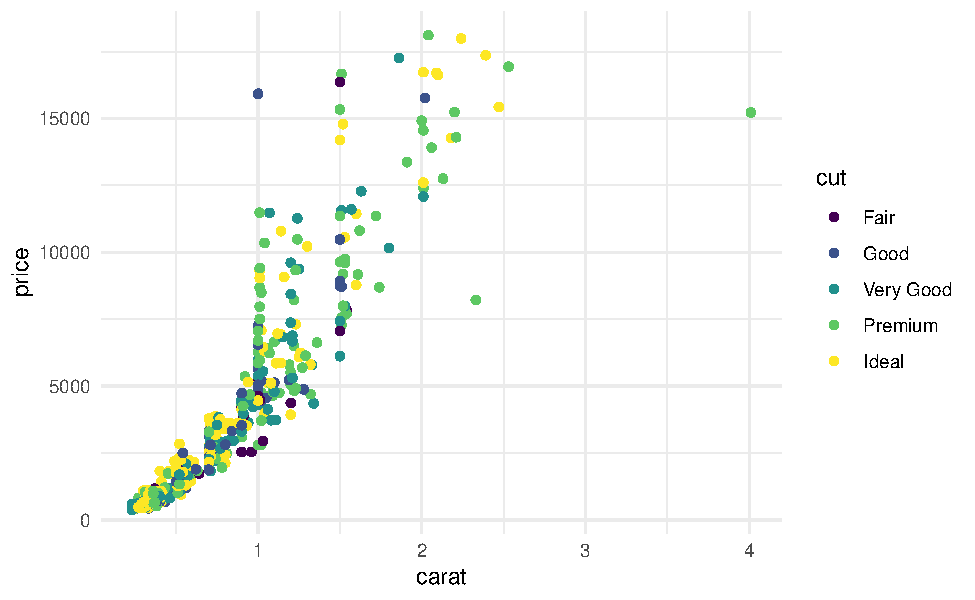
\includegraphics{elsevier_article_files/figure-latex/diamond-plot-1.pdf}
\caption{\label{fig:diamond-plot}this is a figure}
\end{figure}

cross referencing tables \ref{tab:iris}

\begin{table}

\caption{\label{tab:iris}my table}
\centering
\begin{tabular}[t]{r|r|r|r|l}
\hline
Sepal.Length & Sepal.Width & Petal.Length & Petal.Width & Species\\
\hline
5.1 & 3.5 & 1.4 & 0.2 & setosa\\
\hline
4.9 & 3.0 & 1.4 & 0.2 & setosa\\
\hline
4.7 & 3.2 & 1.3 & 0.2 & setosa\\
\hline
4.6 & 3.1 & 1.5 & 0.2 & setosa\\
\hline
5.0 & 3.6 & 1.4 & 0.2 & setosa\\
\hline
5.4 & 3.9 & 1.7 & 0.4 & setosa\\
\hline
\end{tabular}
\end{table}

\hypertarget{installation}{%
\paragraph{Installation}\label{installation}}

If the document class \emph{elsarticle} is not available on your computer,
you can download and install the system package \emph{texlive-publishers}
(Linux) or install the LaTeX package \emph{elsarticle} using the package
manager of your TeX installation, which is typically TeX Live or MikTeX.

\hypertarget{usage}{%
\paragraph{Usage}\label{usage}}

Once the package is properly installed, you can use the document class
\emph{elsarticle} to create a manuscript. Please make sure that your
manuscript follows the guidelines in the Guide for Authors of the
relevant journal. It is not necessary to typeset your manuscript in
exactly the same way as an article, unless you are submitting to a
camera-ready copy (CRC) journal.

\hypertarget{functionality}{%
\paragraph{Functionality}\label{functionality}}

The Elsevier article class is based on the standard article class and
supports almost all of the functionality of that class. In addition, it
features commands and options to format the

\begin{itemize}
\item
  document style
\item
  baselineskip
\item
  front matter
\item
  keywords and MSC codes
\item
  theorems, definitions and proofs
\item
  lables of enumerations
\item
  citation style and labeling.
\end{itemize}

\hypertarget{front-matter}{%
\section{Front matter}\label{front-matter}}

The author names and affiliations could be formatted in two ways:

\begin{enumerate}
\def\labelenumi{(\arabic{enumi})}
\item
  Group the authors per affiliation.
\item
  Use footnotes to indicate the affiliations.
\end{enumerate}

See the front matter of this document for examples. You are recommended
to conform your choice to the journal you are submitting to.

\hypertarget{bibliography-styles}{%
\section{Bibliography styles}\label{bibliography-styles}}

There are various bibliography styles available. You can select the
style of your choice in the preamble of this document. These styles are
Elsevier styles based on standard styles like Harvard and Vancouver.
Please use BibTeX~to generate your bibliography and include DOIs
whenever available.

Here are two sample references: Feynman and Vernon Jr. (1963; Dirac, 1953).

\hypertarget{references}{%
\section*{References}\label{references}}
\addcontentsline{toc}{section}{References}

\hypertarget{refs}{}
\begin{cslreferences}
\leavevmode\hypertarget{ref-Dirac1953888}{}%
Dirac, P.A.M., 1953. The lorentz transformation and absolute time. Physica 19, 888--896. doi:\href{https://doi.org/10.1016/S0031-8914(53)80099-6}{10.1016/S0031-8914(53)80099-6}

\leavevmode\hypertarget{ref-Feynman1963118}{}%
Feynman, R.P., Vernon Jr., F.L., 1963. The theory of a general quantum system interacting with a linear dissipative system. Annals of Physics 24, 118--173. doi:\href{https://doi.org/10.1016/0003-4916(63)90068-X}{10.1016/0003-4916(63)90068-X}
\end{cslreferences}


\end{document}

